We propose to study the method of coinduction. We plan to address the following questions:

\begin{itemize}
\item What is coinduction?
\item What are inductive and coinductive definitions. What is recursion and corecursion.
\item Is coinduction as powerful as induction? Or can we prove theorems that could not be proven otherwise?
\item How can coinduction assist automated reasoning and software verification?
\item What kind of complex systems verification would be assisted by coinduction?
\end{itemize}

\subsection{What is coinduction?}

We will schematically show a derivation of the induction and coinduction principles. For details, refer to \cite{rutten} and \cite{leinster}.

Let $F: Set \to Set$ be a functor.

\subsubsection{(Co)algebras}

\begin{definition}[Algebra]
An algebra is a pair $(A,\alpha)$ where $A \in obj(Set)$ and $\alpha \in \mathcal{A}(F(A),A)$.

\begin{center}
\begin{tikzcd}
F(A) \arrow[r, "\alpha"] & A 
\end{tikzcd}
\end{center}
\end{definition}

\begin{definition}[Coalgebra]
A coalgebra is a pair $(A,\alpha)$ where $A \in obj(Set)$ and $\alpha \in \mathcal{A}(A,F(A))$.

\begin{center}
\begin{tikzcd}
A \arrow[r, "\alpha"] & F(A) 
\end{tikzcd}
\end{center}
\end{definition}

One readily observes that algebra and coalgebra are dual notions.

\begin{example}[Peano view of natural numbers]
	$(\mathbb{N},[zero,succ])$ is an $N$-algebra considering the following structure:
	
	\begin{itemize}
		\item $N: Set \to Set$ is a functor such that $N(X) = 1+X$ where $1 = \{*\}$.
				
		Naturally for $f: X \to Y$, $N(f): 1+X \to 1 + Y$ is given as $N(f) = id + f$.
		
		\item $[zero,succ]: 1+\mathbb{N} \to \mathbb{N}$ is a morphism given by:
		
		 $[zero,succ](n) = 
		 \begin{cases}
		 0 & n = * \\
		 succ(n) & n \neq *
		 \end{cases}$
	\end{itemize}
\end{example}	

\begin{example}[Streams as coalgebras]
	$(\mathbb{N}^{\omega}, \langle \operatorname{head}, \operatorname{tail} \rangle)$ is an $Str$-coalgebra considering the following structure:
	
	\begin{itemize}
		\item $Str: Set \to Set$ is a functor such that $Str(X) = \mathbb{N} \times X$.
		
		Naturally for $f: X \to Y$, $Str(f): \mathbb{N} \times X \to \mathbb{N} \times Y$ is given as $Str(f) = id \times f$.
		
		\item $\langle \operatorname{head}, \operatorname{tail} \rangle: \mathbb{N} \to \mathbb{N} \times \mathbb{N}^{\omega}$ given by:
		
		 $\langle head,tail \rangle(\sigma) = (\sigma(0), \sigma(1) \ldots )$
	\end{itemize}
\end{example}

\subsubsection{Relations between (co)algebras}

We relate two (co)algebras via homomorphisms.

\begin{definition}[Homomorphism of algebras]
Given two F-algebras $(A,\alpha),(B,\beta)$. 

An homomorphism $f$ is a morphism making this diagram commute:	
	
\begin{tikzcd}
F(A) \arrow[d, "\alpha"] \arrow[r, "F(f)"] & F(B) \arrow[d, "\beta"] \\
A \arrow[r, "f"] & B 
\end{tikzcd}
\end{definition}

\begin{definition}[Homomorphism of coalgebras]
Given two F-coalgebras $(A,\alpha),(B,\beta)$.

An homomorphism $f$ is a morphism making this diagram commute:	
	
\begin{tikzcd}
A \arrow[d, "\alpha"] \arrow[r, "f"] & B \arrow[d, "\beta"] \\
F(A) \arrow[r, "F(f)"] & F(B)
\end{tikzcd}
\end{definition}

\subsubsection{Categories of (co)algebras}

\begin{definition}[Categories of (co)algebras]
	$Set^F$ is the category of $F$-algebras:
	
	\begin{itemize}
		\item $obj(Set^F)$ is the class of all $F$-algebras.
		\item $\mathcal{A}(A,B)$ are the $F$-homomorphisms between $F$-algebras $A$ and $B$.
	\end{itemize}

	$Set^F$ is the category of $F$-coalgebras:

	\begin{itemize}
		\item $obj(Set_F)$ is the class of all $F$-coalgebras.
		\item $\mathcal{A}(A,B)$ are the $F$-homomorphisms between $F$-coalgebras $A$ and $B$.
	\end{itemize}
\end{definition}

The notion of subobject translates in this context to the following definition:

\begin{definition}[Subalgebras]
	Let $\mathcal{A} = (A,s)$ be an $F$-algebra and $S \subseteq A$. 
	
	The set $S$ together with a morphism $\beta_S:F(S) \to S$ is a subalgebra if the inclusion $i: S \to A$ is an homomorphism. 
\end{definition}

\subsubsection{Initial algebras and terminal coalgebras}

\begin{definition}[Initial algebra/terminal coalgebra]
	An initial algebra is an initial object in $Set^F$. \\
	A terminal coalgebra is a terminal object in $Set_F$.
\end{definition}

\begin{corollary}
	If an initial F-algebra exists it is unique up to isomorphism. \\
	If a final F-coalgebra exists it is unique up to isomorphism.
\end{corollary}
\begin{proof}
	Consequence of the uniqueness of initial and final objects in a category.
\end{proof}

\begin{example}
$(\mathbb{N},[zero,succ])$ is an initial $N$-algebra.\\
$(\mathbb{N}^{\omega}, \langle \operatorname{head}, \operatorname{tail} \rangle)$ is a final $Str$-coalgebra.
\end{example}

The structure map for initial algebras or final coalgebras is an isomorphism:

\begin{lem}[Lambeck]
The structure map of an initial (final) algebra (coalgebra) is an isomorphism.
\end{lem}
\begin{proof}
The idea is to relate the initial algebra $(A,\alpha)$ with the algebra $(F(A),F(\alpha))$.

\begin{tikzcd}
F(A) \arrow[d, "\alpha"]  & F(F(A)) \arrow[d, "F(\alpha)"] \arrow[l, "F(\alpha)"] \\
A  & F(A) \arrow[l, "\alpha"]
\end{tikzcd}

We then exploit initiality to complete the diagram with some $\beta$:

\begin{tikzcd}
F(A) \arrow[d, "\alpha"] \arrow[r,dashed, "F(\beta)"] & F(F(A)) \arrow[d, "F(\alpha)"] \arrow[l, "F(\alpha)"] \\
A \arrow[r,dashed, "\beta"]  & F(A) \arrow[l, "\alpha"]
\end{tikzcd}

From the first diagram $\alpha$ is an homomorphism of algebras. From the second diagram we see that it must be an isomorphism. Indeed, $\beta \circ \alpha$ is a morphism of algebras with domain and codomain in $A$. Again, by initiality, there can only be one such morphism. But the identity is always a morphism. So, $\beta \circ \alpha = id_A$. 

Finally, $\alpha \circ \beta = F(\beta) \circ F(\alpha) = F(\beta \circ \alpha) = F(id_A) = id_F(A)$ looking at the second diagram.
\end{proof}

\begin{cor}[A functor without initial algebras or final coalgebras]
	The (covariant) powerset functor $\mathcal{P}: Set \to Set$ given by:
	
	\begin{itemize}
		\item For each $X \in Set$, $\mathcal{P}(X) = \{U. U \subseteq X\}$.
		\item For each mapping $f:X \to Y$, $\mathcal{P}(f): \mathcal{P}(X) \to \mathcal{P}(Y)$ assigns $U \mapsto f(U)$.
	\end{itemize}
	
	
	does not have initial algebra or final coalgebra.
\end{cor}
\begin{proof}
	Let's assume that $(A,\alpha)$ is an initial algebra (final coalgebra) for $\mathcal{P}$. By Lambek's lemma we know that $\mathcal{P}(A) \cong A$. Isomorphisms corresponds to bijections in $Set$, and thus, $\mathcal{P}(A)$ should be bijective with $A$. This contradicts Cantor's theorem.
\end{proof}

\subsubsection{F-congruences and F-bisimulations}

The second ingredient needed is F-congruences and F-bisimulations:

\begin{definition}[Congruences]
A relation $R \subseteq S \times T$ is an $F$-congruence if there exists an $F$-algebra structure $(R,\gamma)$ such that the projections $\pi_i$ are $F$-homomorphisms:
	
\begin{tikzcd}
F(S) \arrow[d, "\alpha"] & F(R) \arrow[l, "F(\pi_1)"] \arrow[d, "\gamma",dashed] \arrow[r, "F(\pi_2)"] & F(T) \arrow[d, "\beta"]\\
S  & R \arrow[l, "\pi_1"] \arrow[r, "\pi_2"] &  T
\end{tikzcd}
\end{definition}

\begin{definition}[Bisimulations]
A relation $R \subseteq S \times T$ is an $F$-bisimulation if there exists an $F$-coalgebra structure $(R,\gamma)$ such that the projections $\pi_i$ are $F$-homomorphisms:
	
\begin{tikzcd}
S \arrow[d, "\alpha"] & R \arrow[l, "\pi_1"] \arrow[d, "\gamma",dashed] \arrow[r, "\pi_2"] & T \arrow[d, "\beta"]\\
F(S)  & F(R) \arrow[l, "F(\pi_1)"] \arrow[r, "F(\pi_2)"] &  F(T)
\end{tikzcd}
\end{definition}

\subsubsection{(Co)inductive principles}

Introducing the diagonal set may simplify notation:

\begin{definition}[Diagonal]
	The diagonal of a set $A$, is the set $\Delta(A) = \{(a,a). a \in A\}$
\end{definition}

If $R \subseteq A \times A$ then $\Delta^{-1}(R) = \{a \in A. \Delta(a) \in R\} = \{a \in A. (a,a) \in R\}$

The induction and coinduction principles are formulated as follows:

\begin{thm}[Induction proof principle]
	Every congruence relation on an initial algebra contains the diagonal.
\end{thm}

\begin{thm}[Coinduction proof principle]
	Every bisimulation relation on a final coalgebra contains the diagonal.
\end{thm}


Next we give examples on the natural numbers and streams.

Consider the algebra $(\mathbb{N},[zero,succ])$. We will derive the usual induction principle on natural numbers.

\begin{lem}{N-congruence}
	$R$ is an N-congruence relation iff 
	\begin{itemize}
		\item $(0,0) \in R$
		\item $\forall (n,m) \in \mathbb{N}^2. (n,m) \in R \implies (succ(n),succ(m)) \in R$
	\end{itemize}
\end{lem}

\begin{thm}[Induction on natural numbers]
	The principle of mathematical induction:
	
	$\infer{\forall n. P(n)}{%
		P \subseteq \mathbb{N}
		& P(0)
		& \forall n. P(n) \implies P(succ(n)))
	}$
	 
	is equivalent to the N-induction proof principle:
	
	every $N$-congruence relation on $(\mathbb{N},[zero,succ])$ contains $\Delta(\mathbb{N})$
\end{thm}
\begin{proof}
	$ $\newline
	$\Rightarrow)$ Fix a N-congruence relation $R \subseteq \mathbb{N}^2$ and let $P = \Delta^{-1}(R) = \{n \in \mathbb{N}. (n,n) \in R\}$.
	
	We have $(0,0) \in R$ and thus $P(0)$ holds.
	
	Fix $n$ and assume $P(n)$ holds. This means that $(n,n) \in R$ and therefore $(suc(n), suc(n)) \in R$ which implies $P(suc(n))$. 
	
	By the principle of mathematical induction. This means that $\forall n \in \mathbb{N}. (n,n) \in R$ which implies that $\Delta(\mathbb{N}) \subseteq R$. 
	
	$\Leftarrow)$ Fix $P \subseteq \mathbb{N}$ and assume $P(0)$ and $\forall n. P(n) \implies P(succ(n))$.
	
	Define $R = \{(m,n) \in \mathbb{N}^2. P(m) \land P(n)\}$. $R$ is an N-congruence since:
	
	\begin{itemize}
		\item $(0,0) \in R$ as $P(0)$ holds.
		\item $(m,n) \in R \implies P(m) \land P(n) \implies P(succ(m)) \land P(succ(n)) \implies (succ(m),succ(n)) \in R$
	\end{itemize}

	By the N-induction principle, we know that $\Delta(\mathbb{N}) \subseteq R$ and thus, $\forall n. P(n)$ holds.
\end{proof}

We could wonder if the principle of complete mathematical induction:

$\forall P \subseteq \mathbb{N}. (P(0) \land (\forall n. (\forall m < n. P(m)) \implies P(n))) \implies \forall n. P(n)$

also has a categorical interpretation? In any case, it is equivalent to mathematical induction. On the other hand, a direct derivation could be obtained by modifying the predicate $P$ and relation $R$ provided above. 

\begin{lem}
	$R \subseteq \mathbb{N}^{\omega} \times \mathbb{N}^{\omega}$ on $(\mathbb{N}^{\omega}, \langle \text{head}, \text{tail} \rangle)$ is a Str-bisimulation iff:
	
	$\forall (\sigma,\tau) \in R. \text{head}(\sigma) = \text{head}(\tau) \land (\text{tail}(\sigma), \text{tail}(\tau)) \in R$
\end{lem}


\begin{thm}[Coinductive proof principle on Streams]
	The coinductive proof principle applied to the final coalgebra $(A^{\omega}, \langle \text{head}, \text{tail} \rangle)$ takes the following form:
	
	\[
	\infer{s = s'}{%
		R \subseteq A^{\omega} \times A^{\omega}
		& R \; s \; s'
		&
		\qinfer{\forall s_1,s_2}
		{\func{head}(s_1) = \func{head}(s_2) \land R(\func{tail}(s_1), \func{tail}(s_2))}
		{R \; s_1 \; s_2}
	}
	\]
\end{thm}

TODO: An example of proof through coinduction

\subsection{Functional programming and (co)algebras}

Coinduction has been studied in software verification \cite{leino} and theorem proving \cite{blanchette}. We want to explore the implementation of coinduction in Isabelle \cite{blanchette} \cite{sweden}. For that we would like to understand what is a (co)datatype in categorical terms \cite{course} (lecture 8, point 4) \cite{mario}. In this section, we will also investigate how are common functional programming patterns seen from the point of view of category theory.  

\begin{definition}[Polynomial functor]
	Let $A_1, \ldots , A_k$ be sets and $n_1, \ldots n_k \in \mathbb{N}$. 
	
	A functor $F: Set \to Set$ given by: $$F(X) = A_1 \times X^{n_1} + \ldots + A_k \times X^{n_k}$$ is said to be polynomial.
\end{definition}

\begin{remark}
	Interpreted in $Set$, $\times$ is the cartesian product and $+$ is the disjoint union. 
\end{remark}

\begin{definition}[(Co)datatype]
	A datatype is the initial algebra of a polynomial functor. \\
	A codatatype is the final algebra of a polynomial functor.
\end{definition}


Given a polynomial functor $F$ with initial algebra $(T,c)$ where: $$c: A_1 \times T^{n_1} + \ldots + A_k \times T^{n_k} \to T$$ since $+$ corresponds to a disjoint union, we can write $c = [c_1,\ldots,c_k]$ with: $$c_i: A_i \times T^{n_i} \to T$$ Moreover, $T$ is completely determined by the $c_i$ by Lambek's lemma. 

In a programming language, the corresponding constructs are written as follows:

\begin{align*}
datatype \; T &= c_1 \; of \; A_1 \times T^{n_1} \\
&\;\;\vdots \notag \\
&| = c_k \; of \; A_k \times T^{n_k} \\
\end{align*}
\begin{align*}
codatatype \; T &= c_1 \; of \; A_1 \times T^{n_1} \\
&\;\;\vdots \notag \\
&| = c_k \; of \; A_k \times T^{n_k} \\
\end{align*}

\begin{remark}
	The non-categorical interpretation, defines a (co)datatype as the smallest(greatest) set closed by the constructors (destructors).
\end{remark}

\begin{example}[(Co)datatypes by iteration]
	By checking initiality of certain algebras we get to definitions by iteration. 
	
	For instance, let's check that $(\mathbb{N},zs)$ is an initial algebra.
	
	We show that there exists a unique $f$ such that the following diagram commutes:
	
	\begin{tikzcd}
	1 + \mathbb{N} \arrow[r, "N(f)"] \arrow[d, "zs",swap] & 1+X \arrow[d, "\alpha"] \\
	\mathbb{N} \arrow[r, "f",swap] & X
	\end{tikzcd}
	
	That is, $\alpha \circ N(f) = f \circ zs$ where $zs = [zero,succ]$. Equivalently:
	
	\begin{itemize}
		\item $f(0) = \alpha(*)$
		\item $\forall x \in \mathbb{N}. f(x+1) = \alpha(f(x))$ 	
	\end{itemize}

	By natural induction, there is a unique $f$ satisfying this definition.	Since $f$ is defined iterating over $\alpha$, it is sometimes denoted $iter(\alpha)$ \cite{geuvers2007iteration}. More generally, we can see our initial algebra endowed with an iterator mapping $iter$ sending each $\alpha$ to the function $f$ it defines. 
	
	Dually, by checking terminality of certain coalgebras we get definitions by coiteration.
	
	We show that there exists a unique $f$ such that the following diagram commutes:
	
	\begin{tikzcd}
		\mathbb{N}^{\omega} \arrow[d, "ht",swap] & X \arrow[l, "f",swap] \arrow[d, "\alpha"] \\
		\mathbb{N} \times \mathbb{N}^{\omega} & \mathbb{N} \times X \arrow[l, "Str(f)",swap]
	\end{tikzcd}

	That is, $ht \circ f = Str(f) \circ \alpha$ where $ht = [head,tail]$. Equivalently:
	
	\begin{itemize}
	\item $head(f(x)) = \alpha_1(x)$
	\item $tail(f(x)) = f(\alpha_2(x))$ 	
	\end{itemize}

	which defines the stream $f(x) = \alpha_1(x) \; \alpha_1(\alpha_2(x)) \; \alpha_1(\alpha_2^ 2 (x)) \ldots$. Since $f$ is defined iterating over $\alpha$, it is sometimes denoted $coiter(\alpha)$ \cite{geuvers2007iteration}. More generally, we can see our terminal coalgebra endowed with a coiterator mapping $coiter$ sending each $\alpha$ to the function $f$ it defines. 		
\end{example}

It is worth noting from the examples above that the structure map of a (co)algebra indicates the basic operations that are available for the (co)datatype, while the initiality property is essential in proving facts about the (co)datatype. \cite{smyth1982category}

Definitions by iteration provide means of computing functions $f$ starting from an initial value $*$ and then applying iteratively the same function $\alpha$ to the obtained computations. We can also model other definitional paradigms, namely, primitive recursion and case analysis. 

\begin{lemma}[Primitive recursion on initial algebras]
	Let $(A,in,iter)$ be an initial algebra and $g: T(B\times A) \to A$. 
	
	There is a unique morphism $h$ making the following diagram commute:
	
	\begin{tikzcd}
		T A \arrow[d, "in",swap] \arrow[dashed]{r}{T \langle h,id \rangle} & T(B \times A) \arrow[d,"g"] \\
		A \arrow[r, "h",swap, dashed] & B
	\end{tikzcd}

	In fact, $h = \pi_1 \circ iter\langle g, in \circ T(\pi_2)\rangle$
\end{lemma}
\begin{proof}
	See lemma 2.5 in \cite{geuvers2007iteration}.
\end{proof}

\begin{example}[Primitive recursion on natural numbers]
The scheme for primitive recursion on natural numbers looks as follows:

\begin{itemize}
	\item $h(0) = g_1(*)$
	\item $h(succ(n)) = g_2(h(n), n)$ 
\end{itemize}

This can be modeled using $T = N, A = B = \mathbb{N}$. 

The predecessor function is often quoted to be easier to be defined through recursion than by iteration.
\end{example}

Since $h$ is defined recurring to $g$, we write it $h = rec(g)$ and for an initial algebra we can establish a mapping $rec$ assigning to each extra parameter supplier $g$, the function $h$ it defines.

\begin{lem}[Case analysis on initial algebras]
	Let $(A,in,iter)$ be an initial $T$-algebra and $g:T(A) \to B$.
	
	There exists a unique morphism $h$ making the following diagram commute:
	
	\begin{tikzcd}
		T A \arrow[r, "in",swap] \arrow[swap]{dr}{g} & A \arrow[d,"h",dashed] \\
		 & B
	\end{tikzcd}
\end{lem}

\begin{example}[Case analysis on natural numbers]
	Case analysis over natural numbers can be seen as follows:
	
	\begin{itemize}
		\item $h(0) = g_1(*)$
		\item $h(succ(n)) = g_2(n)$
	\end{itemize}

	This corresponds to the above definitions with $T = N, A = \mathbb{N}$.
\end{example}


TODO: corecursion, cocase analysis


\subsection{Building initial and final algebras}

Our goal now is to investigate different approaches to build datatypes and codatatypes in programming language theory. From the examples above it is reasonable to ask the following question: does the initial/final (co)algebra of a polynomial endofunctor always exist? If so, can we compute it?

\subsubsection{Adamek's and Barr's theorems}

We consider a generalization of Kleene's fixed-point theorem. It may be interesting to include some notation so that we understand better the construction involved. 

\begin{thm}[Adamek-Barr]
	The two statements below are dual of each other:
	
	\begin{itemize}
		\item Let $\mathcal{C}$ be a category with initial object $0$ and colimits for any $\omega$-chain. If $F: \mathcal{C} \to \mathcal{C}$ preserves the colimit of initial $\omega$-chain, then the initial $F$-algebra is $\mu(F) = \text{colim}_{n < \omega} F^n 0$.
		\item Let $\mathcal{C}$ be a category with terminal object $1$ and limits for any $\omega^{op}$-chain. If $F: \mathcal{C} \to \mathcal{C}$ preserves the limit of terminal $\omega^{op}$-chain, then the terminal $F$-coalgebra is $\nu(F) = \text{lim}_{n < \omega^{op}} F^n 1$.
	\end{itemize}
	
\end{thm}
\begin{proof}
	We follow here the proof in Jacobs \cite{jacobs2005introduction} who does it for the second case.
	
	Assume there is a limit $Z$ of the chain starting at the final object:
	
	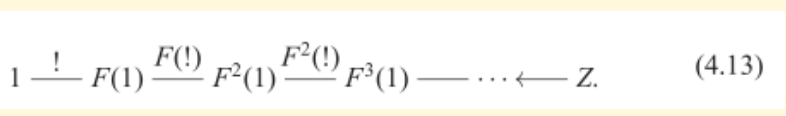
\includegraphics[width=0.5\textwidth]{img/chain}
	
	If $F$ preserves $\omega$-limits then $Z \to F(Z)$ is a final coalgebra.
	
	Actually we only need that $F$ preserves the limit of this chain. 
	
	Assume that $Z$ in the above diagram is a limit with $\xi_n:Z \to F^n(1)$ the corresponding commutative cone satisfying that $F^n(!) \circ \xi_{n+1} = \xi_n$. 
	
	Applying $F$ to the cone and the above equations yields another commutative cone with base $F(Z)$  and components $F(\xi_n):F(Z) \to F^{n+1}(1)$. The limit of this cone is $F(Z)$ since by assumption $F$ preserves limits.
	
	Now, it should be observed that indeed, $Z$ can be used as the base of a shorter cone starting at $F(1)$. Since, $F(Z)$ is the limit of such chain we get a unique homomorphism $\xi: Z \to F(Z)$. 
	
	Incidentally one can also extend the chain whose base is $F(Z)$ into a chain starting in $1$ this is by using the unique properties of terminal object $1$. Commutativity holds and at the end we get another homomorphism $\xi': F(Z) \to Z$. It follows that $\xi \circ \xi'$ and $\xi' \circ \xi$ are homomorphisms on final cones. This implies that they are the identity.
	
	In summary, we can also say that $\xi$ is an isomorphism with inverse $\xi'$. The homomorphism condition yields the equation $F(\xi_n) \circ \xi \stackrel{1}{=} \xi_{n+1}$
	
	Then he goes on to show that $(Z,\xi)$ is a final coalgebra. 
	
	For an arbitrary coalgebra $c:Y \to F(Y)$ we can form a collection of maps $c_n: Y \to F^n(1)$ via:
	
	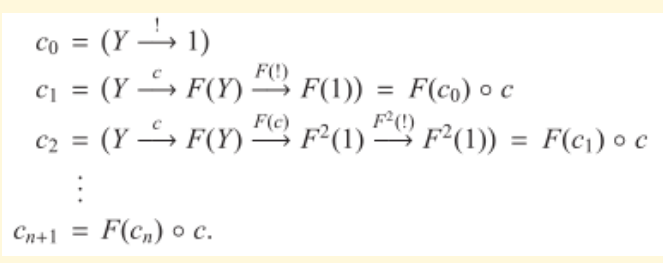
\includegraphics[width=0.5\textwidth]{img/mappings}
	
	The base $Y$ and the maps $c_n$ form a commutative cone. To see this it is useful to distinguish between $!_y$ and $!_1$ which signals to what chain does the unique morphism belong to. By induction:
	
	Base case: $c_0 = !_1 \circ c_1$. This holds directly because of the uniqueness of $c_0 = !_y$. 
	
	Inductive case: let's assume that $c_{n-1} = F^{n-1}(!_1) \circ c_{n}$.  We have to show that $c_{n} = F^{n}(!_1) \circ c_{n+1}$.
	
	Indeed,from the induction hypothesis we get that $F(c_{n-1}) \stackrel{*}{=} F^n(!_1) \circ c_n$ and the right hand side then is:
	
	$F^{n}(!_1) \circ c_{n+1} = F^{n}(!_1) \circ F(c_n) \circ c \stackrel{*}{=} F(c_{n-1}) \circ c = c_n$
	
	As a consequence, since $Z$ is the base of the initial cone this yields a unique cone homomorphism $h: Y \to Z$ with $\xi_n \circ h \stackrel{3}{=} c_n$
	
	
	Let's check that $h$ is an homomorphism of coalgebras, i.e satisfies $\xi \circ h = F(h) \circ c$.
	
	Note at this point that while $\xi \circ h$ is a cone homomorphism, it is not necessary the case that $F(h) \circ c$ is. In particular, we don't have that $c$ is a cone homomorphism.
	
	We would be done if we check that both behave the same on the components of the cone with base $F(Z)$. This would imply that $F(h) \circ c$ is also an homomorphism. Since $F(Z)$ is a limit there can be only one such homomorphism and the equality follows. Now:
	
	$F(\xi_n) \circ \xi \circ h \stackrel{1}{=} \xi_{n+1} \circ h \stackrel{3}{=} c_{n+1} \stackrel{2}{=} F(c_n) \circ c \stackrel{3}{=} F(\xi_n) \circ F(h) \circ c$
	
\end{proof}

\begin{cor}
	Any polynomial functor on $Set$ admits an initial algebra and a final coalgebra.
\end{cor}
\begin{proof}
	Check with corollary 4.6.3 in \cite{jacobs2005introduction}.
\end{proof}


In the context of Isabelle these constructions are however, not suited because arbitrary limits require reasoning about infinite type families which is not available in HOL.


\subsubsection{Bounded endofunctor theorem}


The finite powerset is not continuous but has a final coalgebra. Hence we shall need
more powerful techniques to cover a larger class of functors. 




